\section{Introduction}


%%%%%%%%%%%%%%%%%%%%%%%%%%%%%%%%%%%%%%%%%%%%%%%%%%%%%%%%%%%%%%%%%%%%%%%%%%%%%%%
\section{Methodology}

This is Euler's homogeneity equation

\begin{equation}
  \label{eq_euler_homogeneity}
  (x - x_c)\partial_x f + (y - y_c)\partial_y f + (z - z_c)\partial_z f
  = (b - f)\eta
  \ ,
\end{equation}

\noindent
in which $(x_c, y_c, z_c)$ are the coordinates of the magnetic field source,
$b$ is the base level representing a constant shift in the signal, and $\eta$
is the structural index corresponding to the nature of the source. You can
reference the equation in the text like this:
Equation~\ref{eq_euler_homogeneity}.




%%%%%%%%%%%%%%%%%%%%%%%%%%%%%%%%%%%%%%%%%%%%%%%%%%%%%%%%%%%%%%%%%%%%%%%%%%%%%%%
\section{Results}


\subsection{Method demonstration with a single window}

\begin{figure}[tb!]
\centering
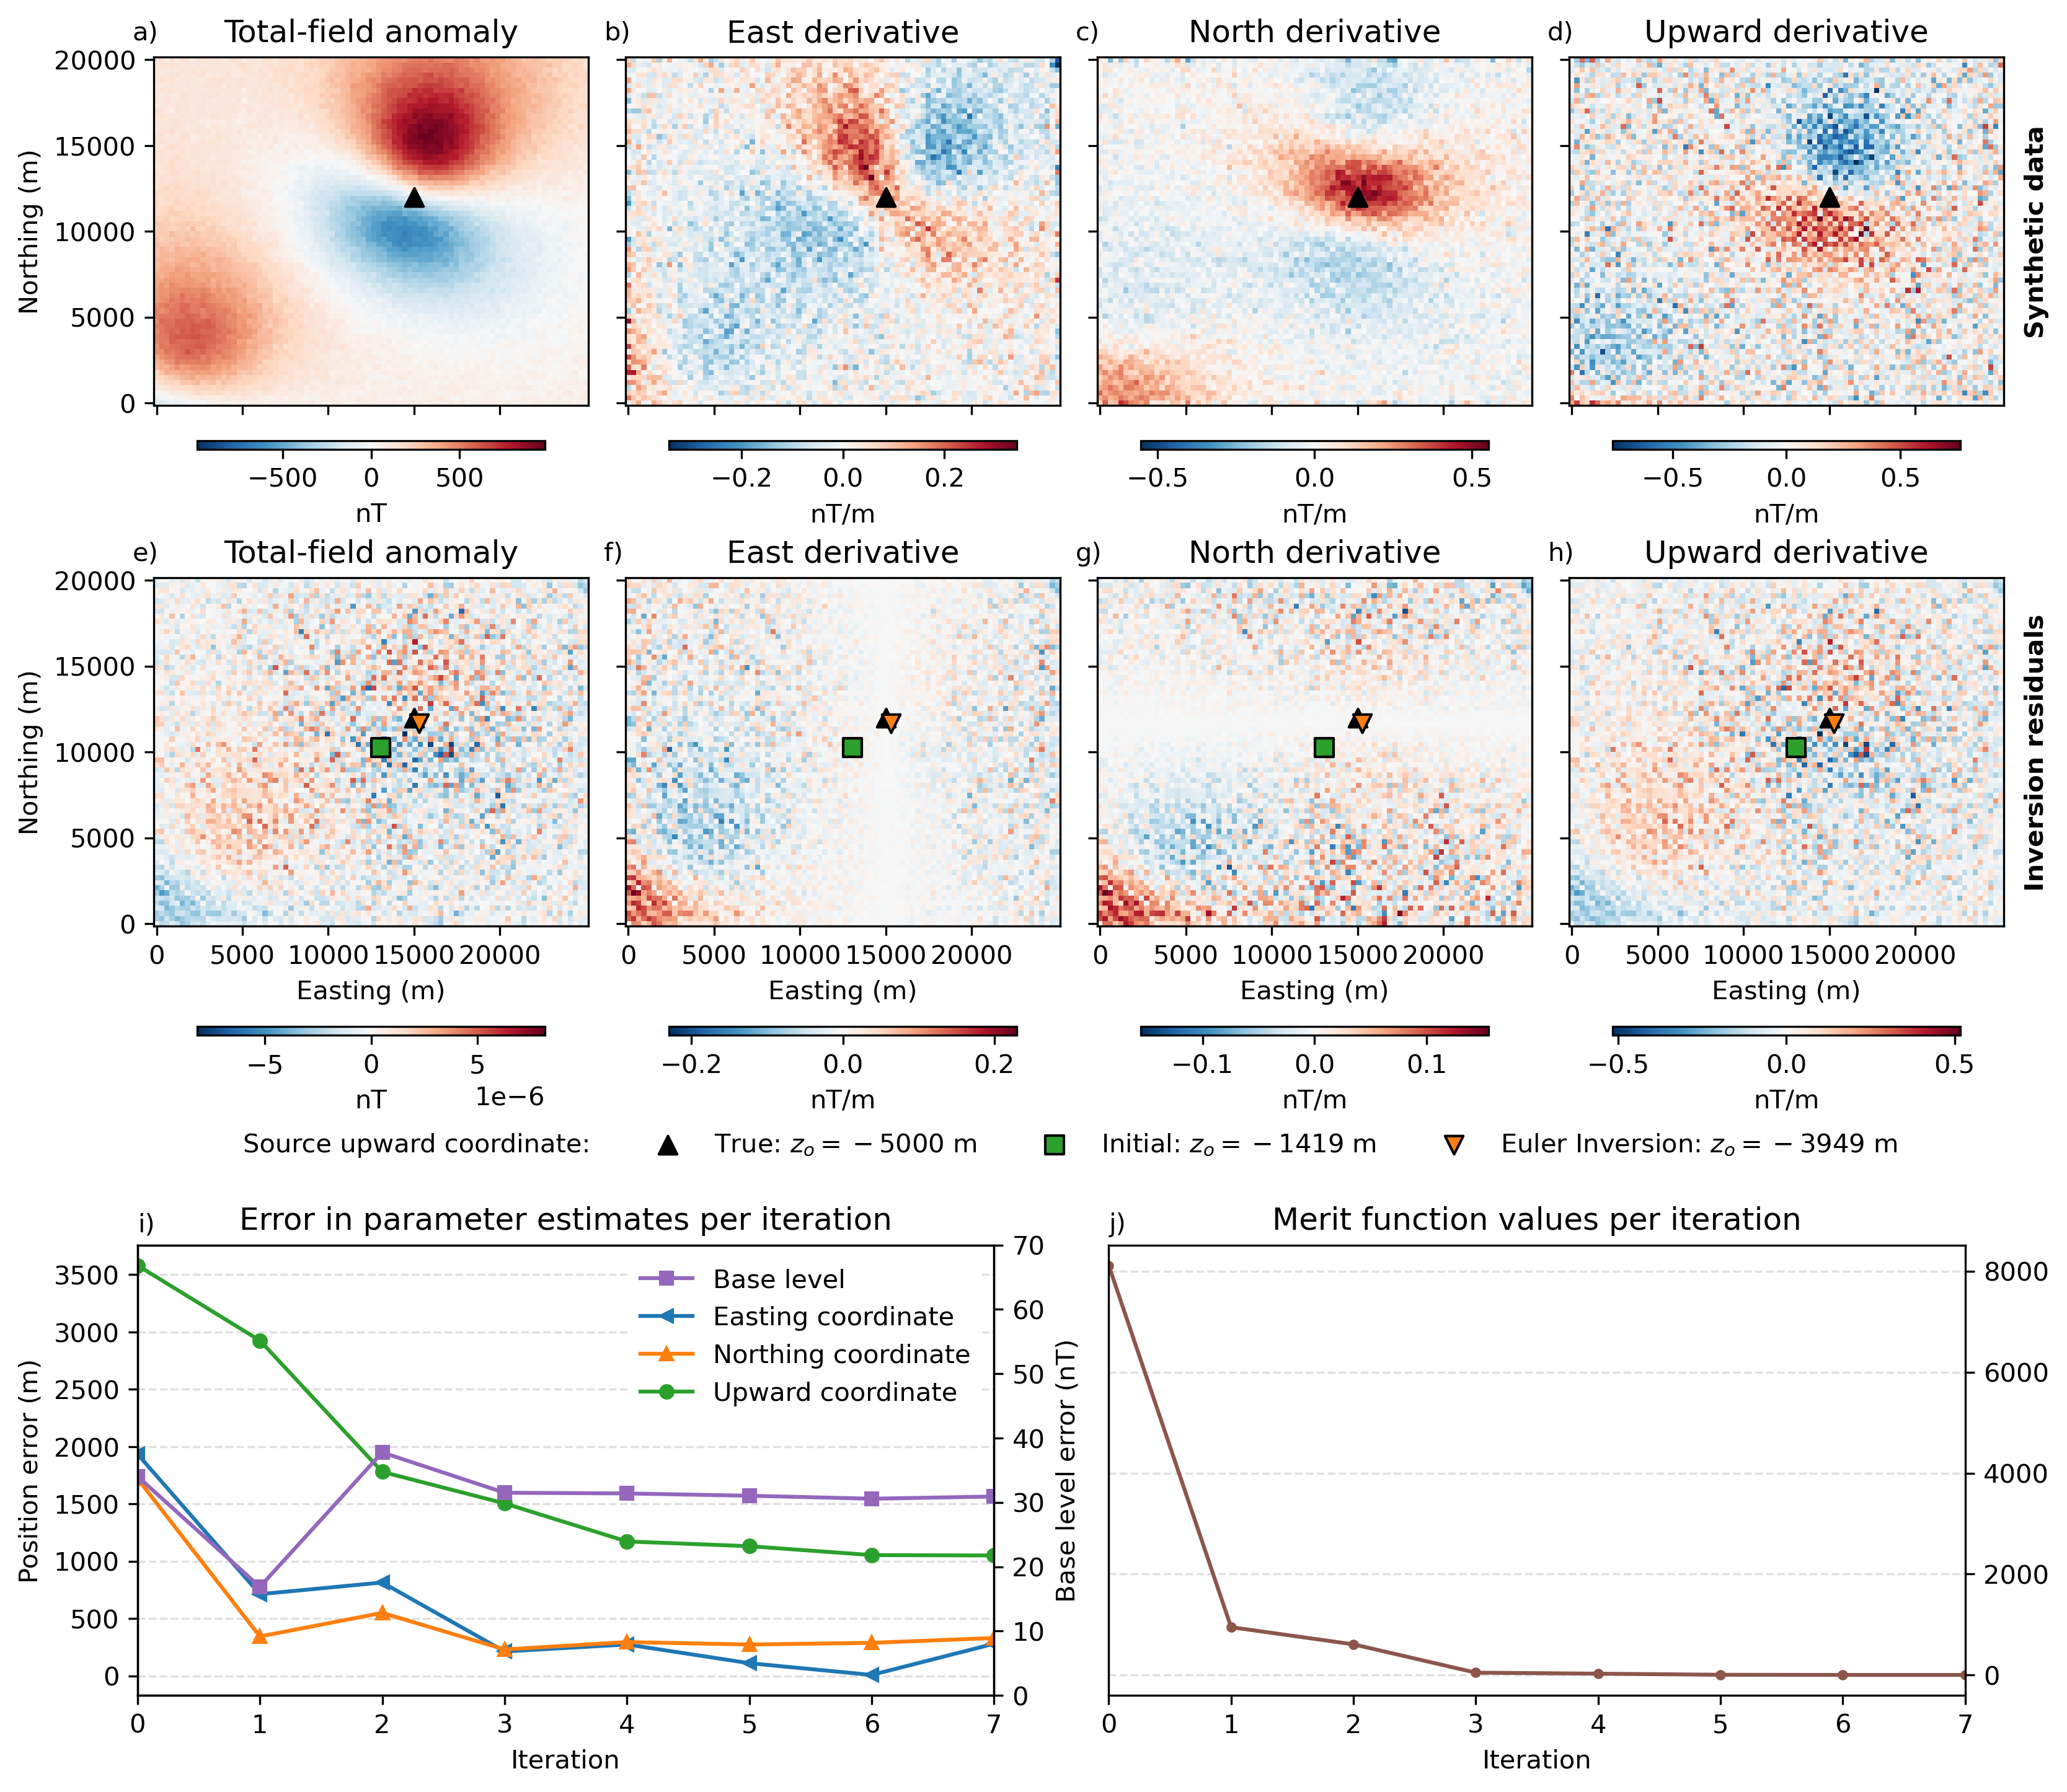
\includegraphics[width=1\linewidth]{figures/synthetic-proof-of-concept.png}
\caption{
  \lipsum[1]
}
\label{fig:proof}
\end{figure}


\subsection{Effect of random noise}

\begin{figure}[tb!]
\centering
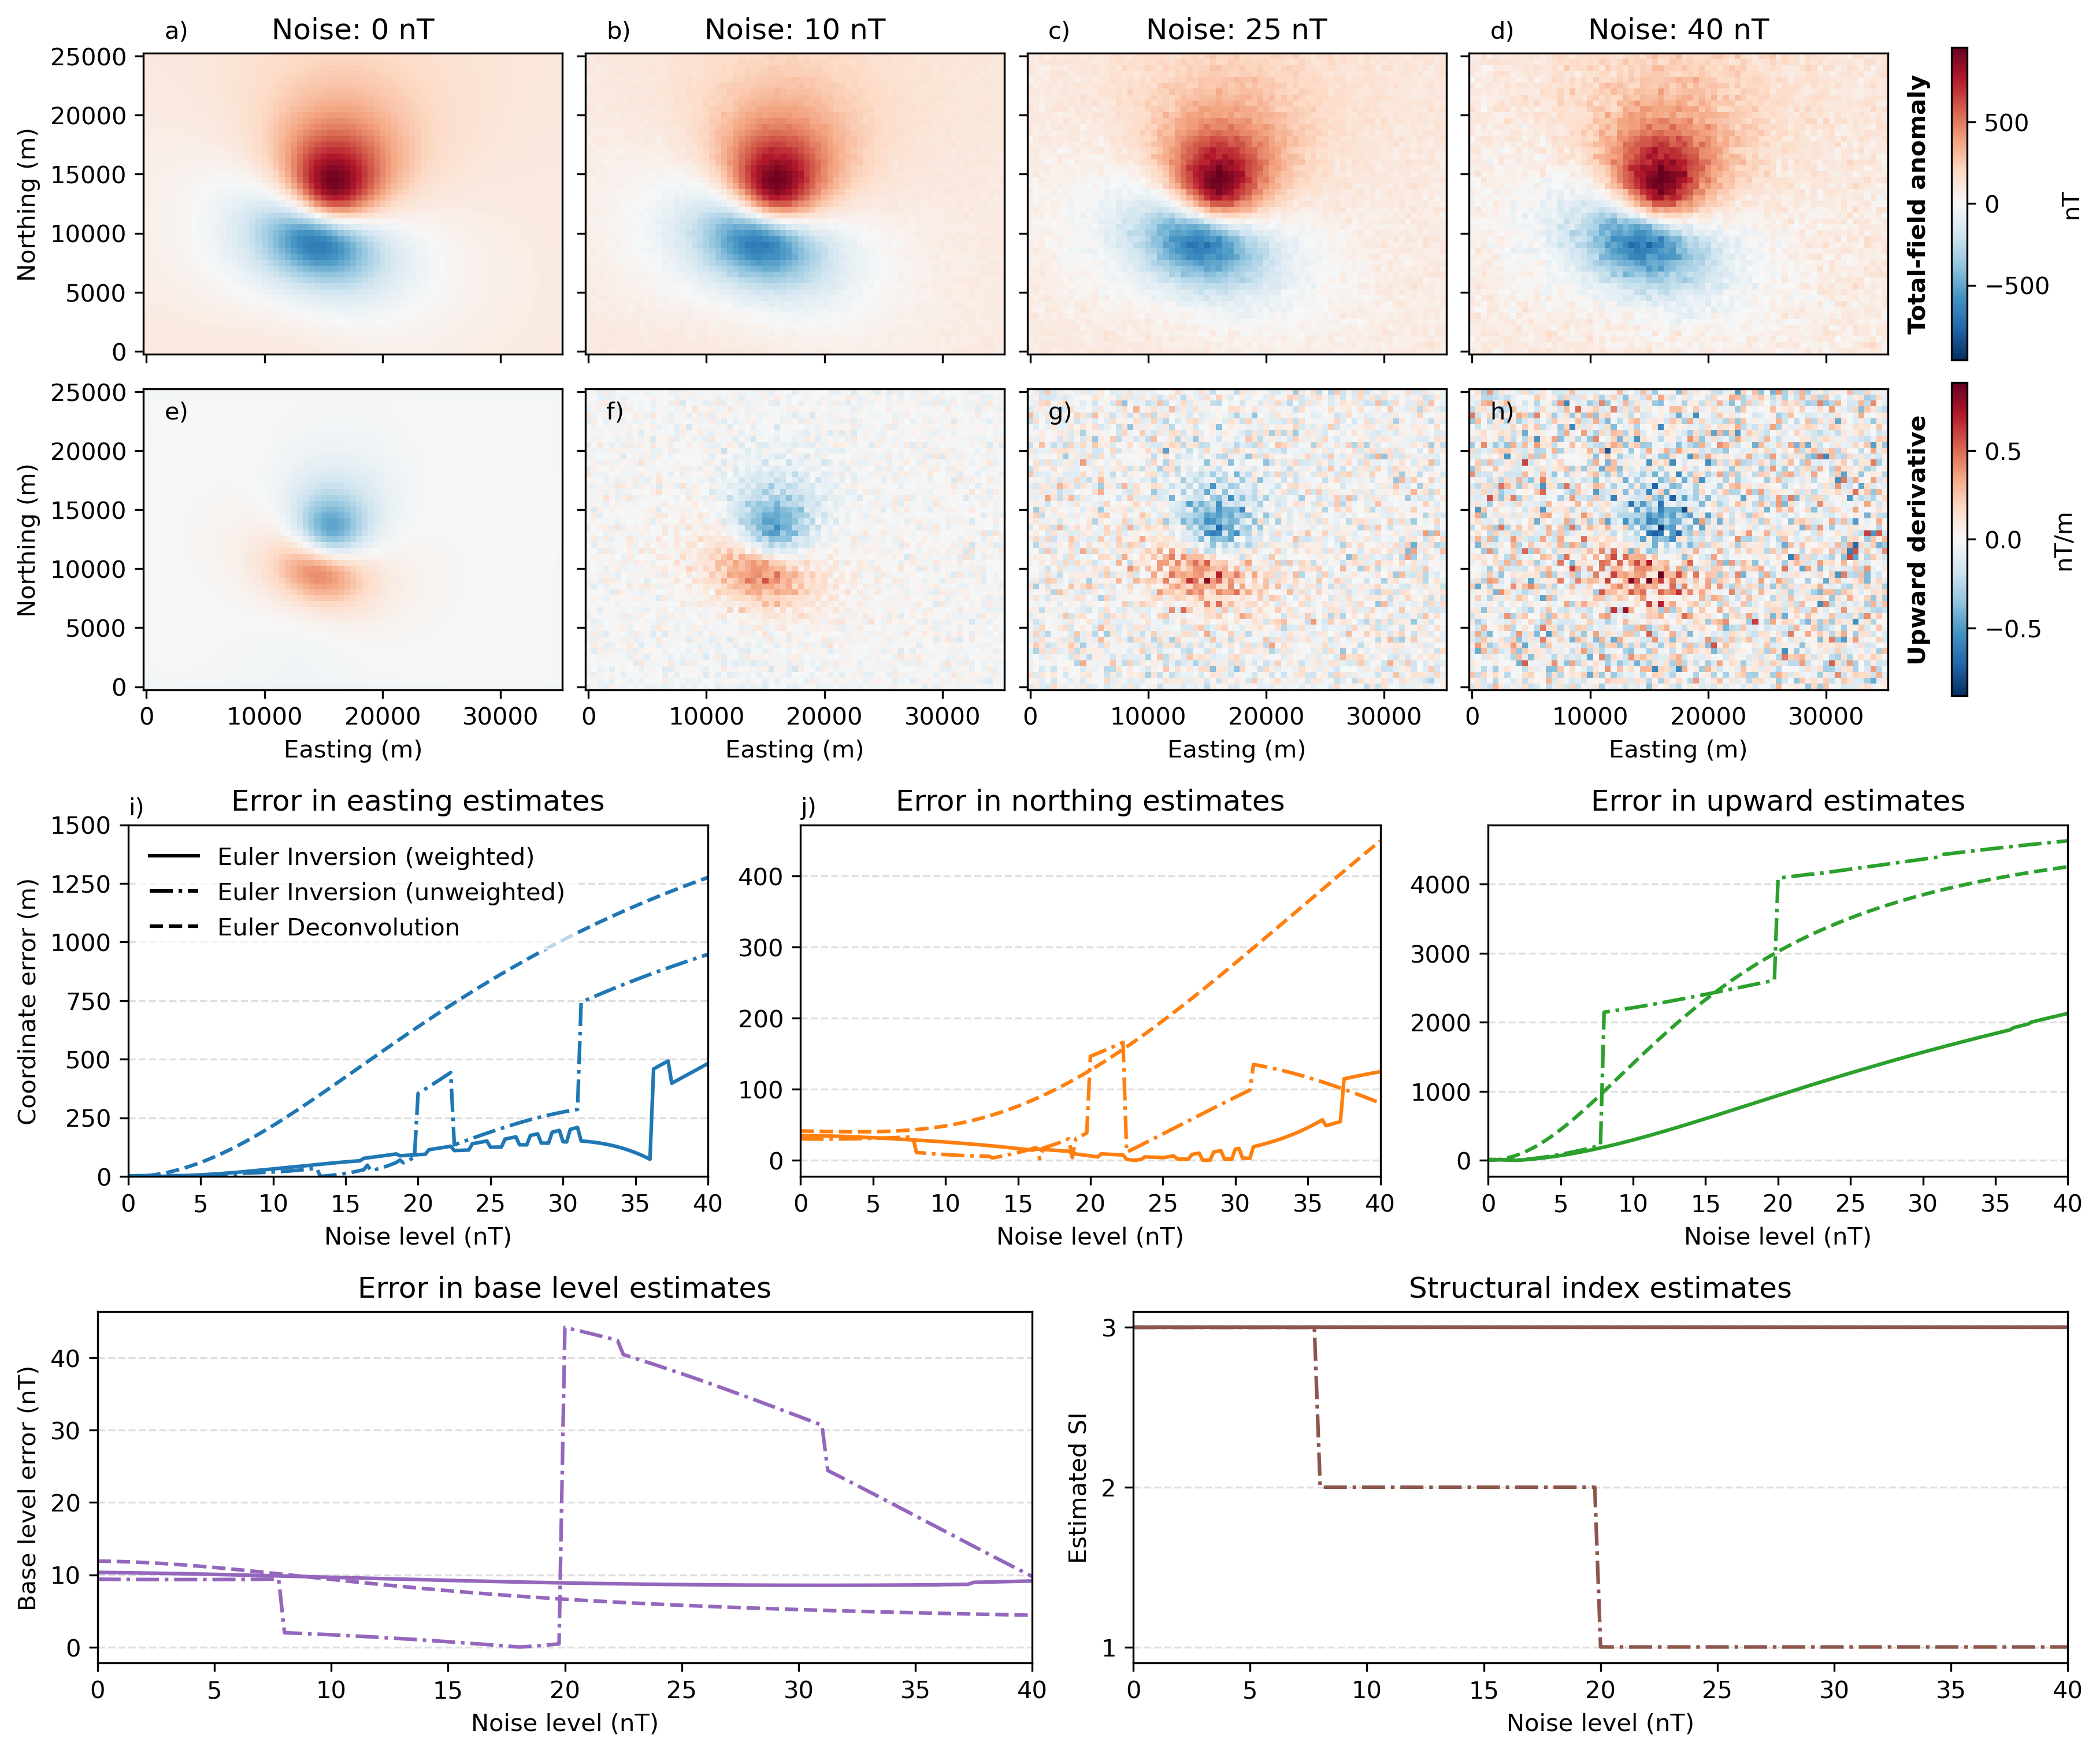
\includegraphics[width=1\linewidth]{figures/synthetic-noise-levels.png}
\caption{
  \lipsum[1]
}
\label{fig:noise}
\end{figure}

\subsection{Effect of SI on multiple sources}

\begin{figure}[tb!]
\centering
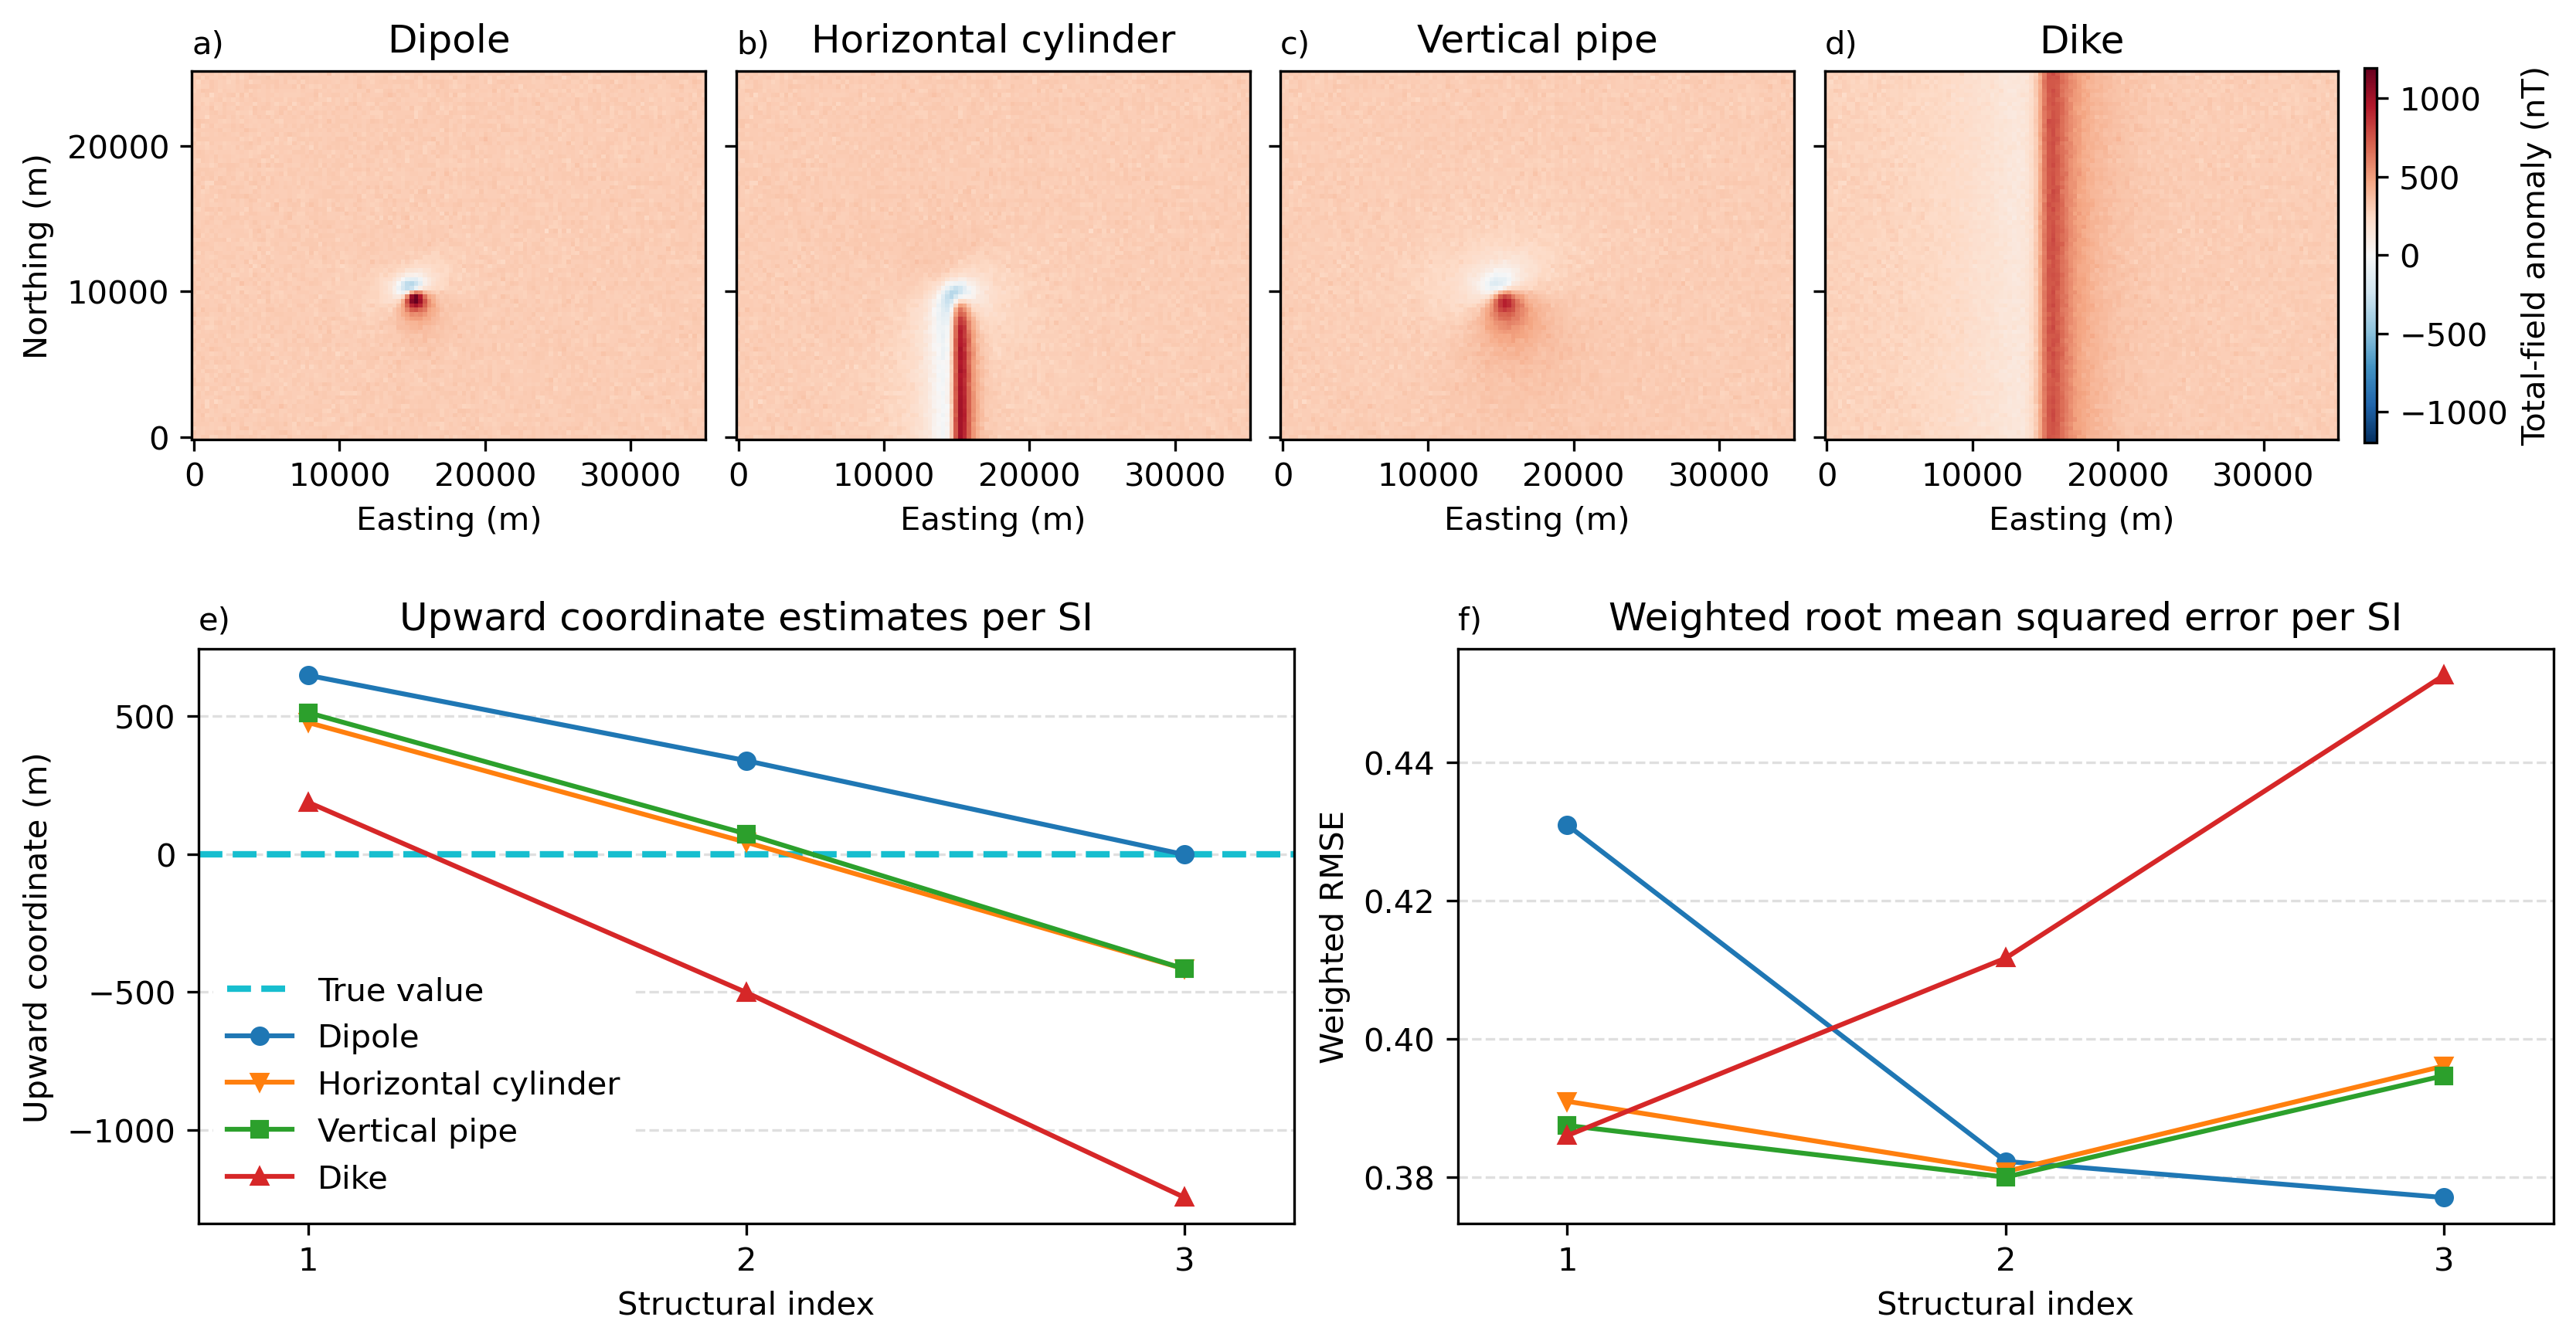
\includegraphics[width=1\linewidth]{figures/synthetic-structural-index.png}
\caption{
  \lipsum[1]
}
\label{fig:si}
\end{figure}

\subsection{Windowing procedure with multiple sources}

\begin{figure}[tb!]
\centering
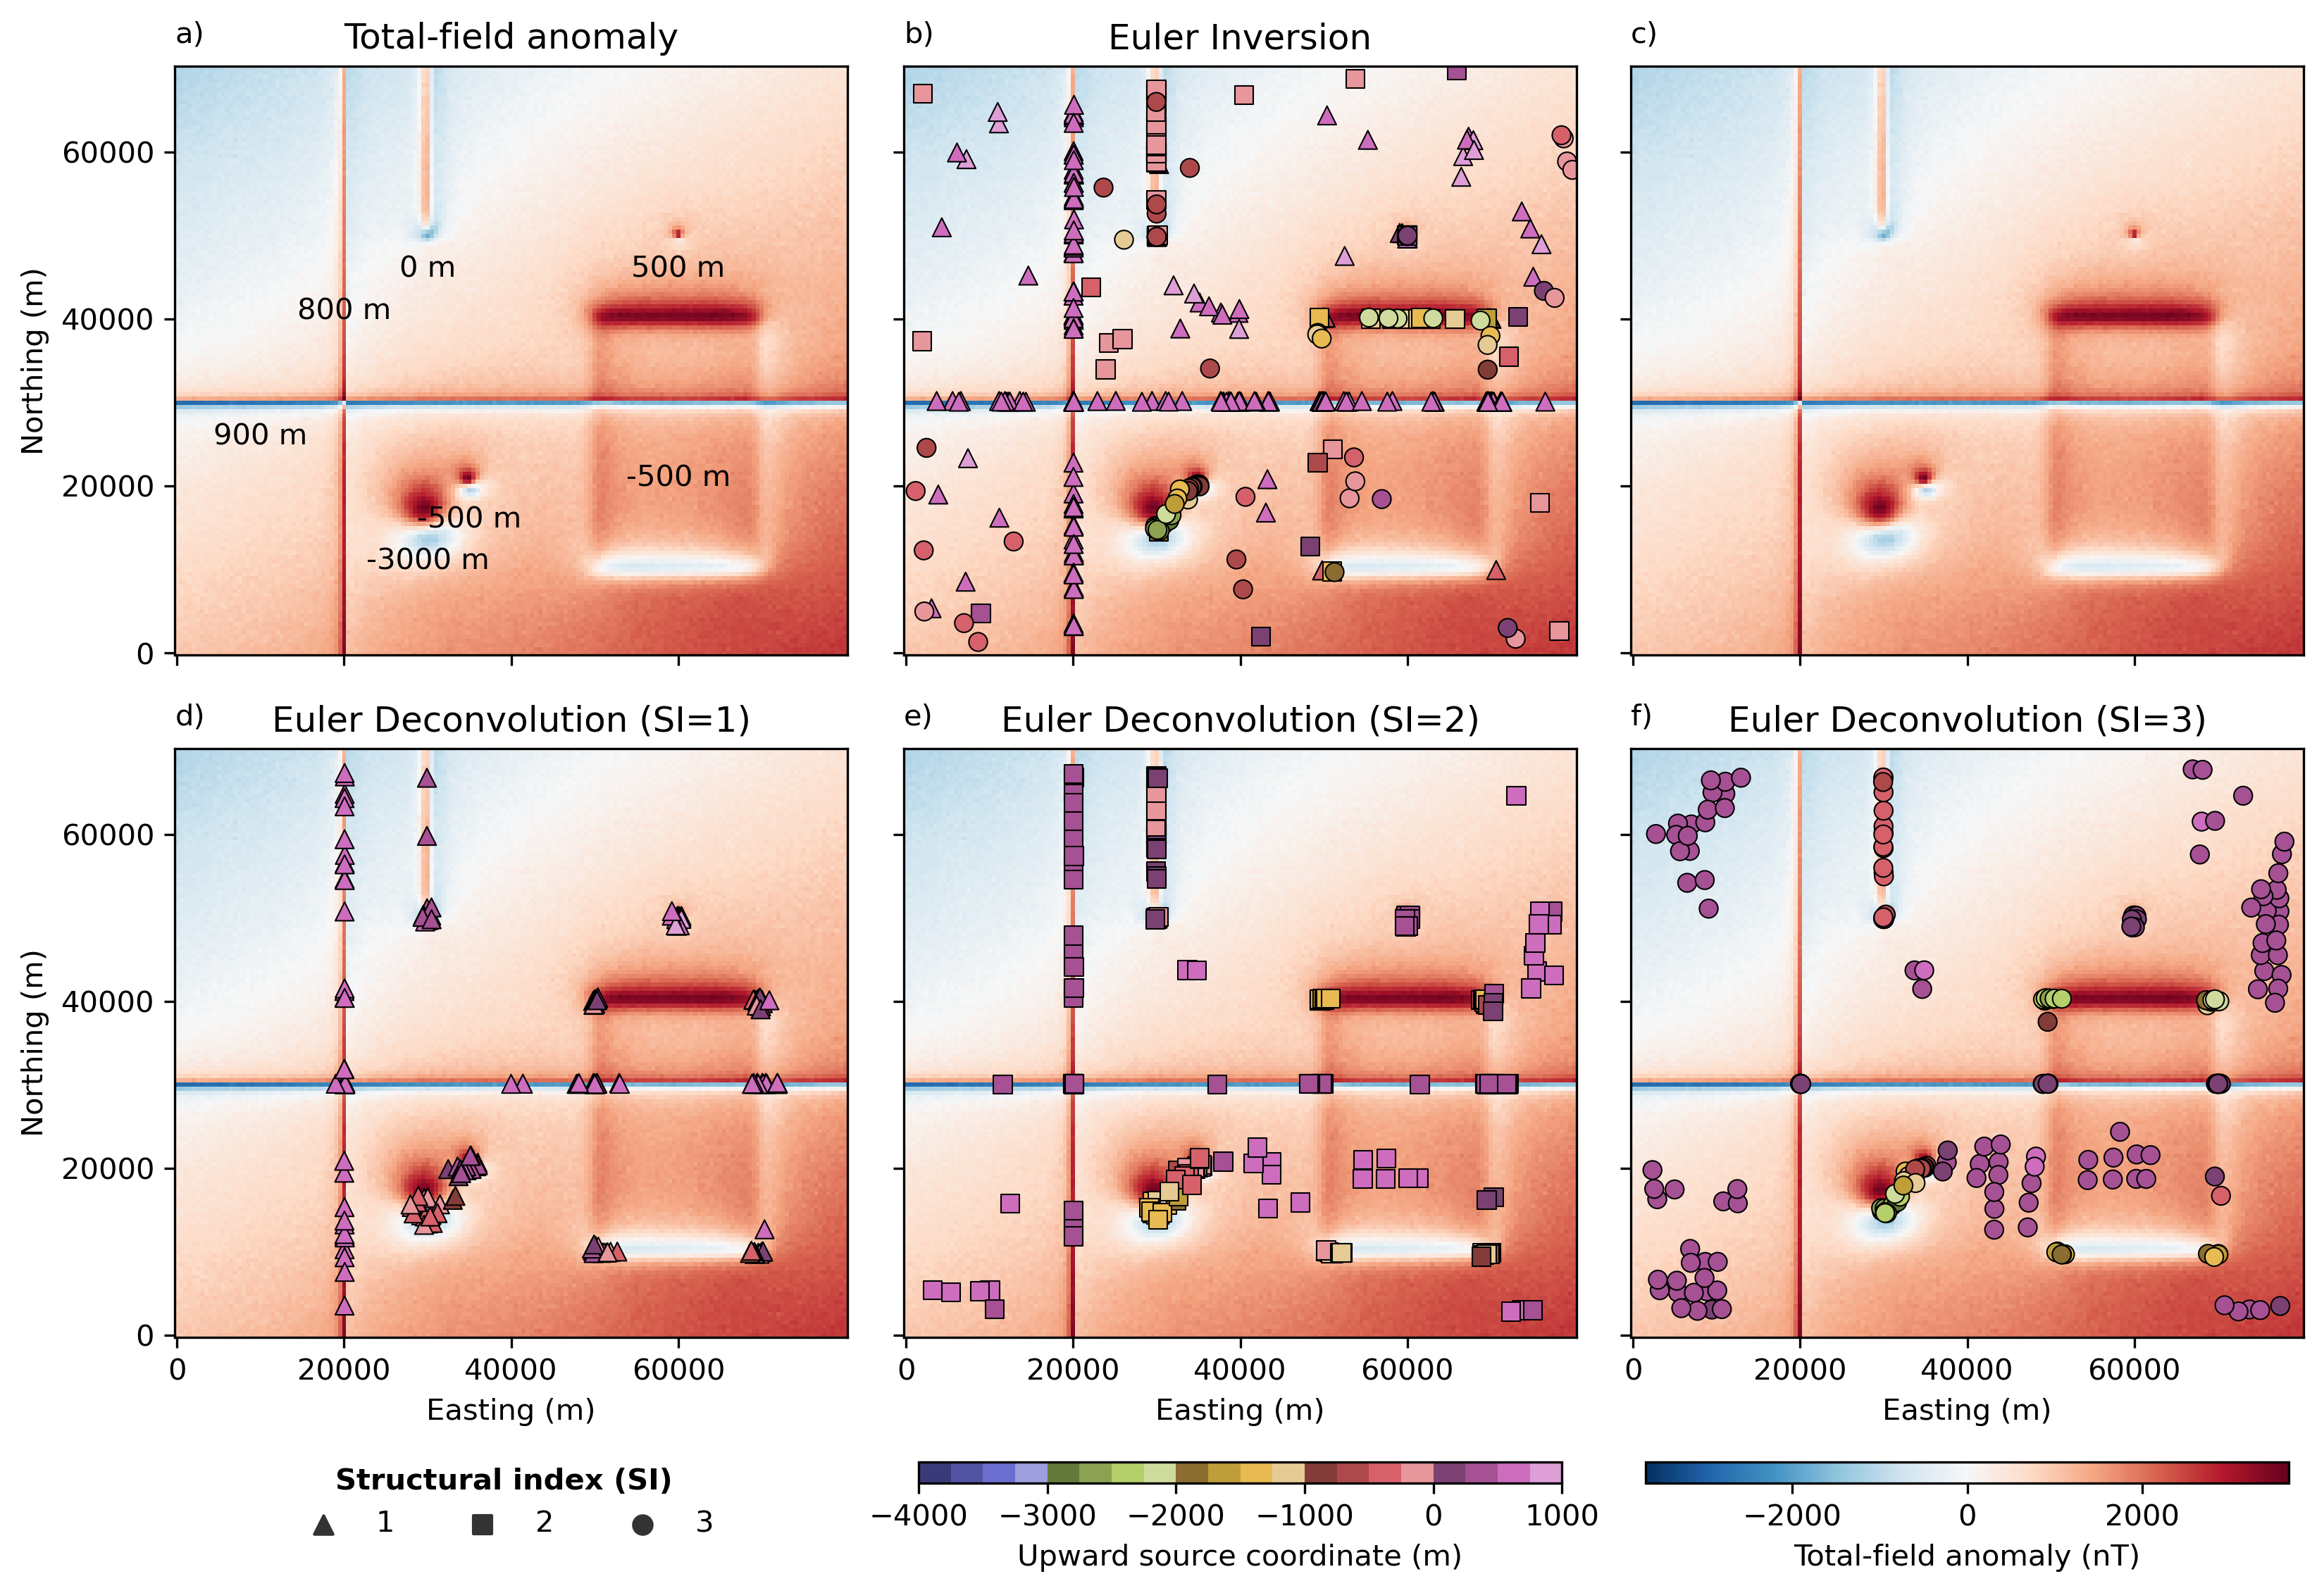
\includegraphics[width=1\linewidth]{figures/synthetic-windows.png}
\caption{
  \lipsum[1]
}
\label{fig:windows}
\end{figure}

\subsection{Aeromagnetic data from Rio de Janeiro}

%%%%%%%%%%%%%%%%%%%%%%%%%%%%%%%%%%%%%%%%%%%%%%%%%%%%%%%%%%%%%%%%%%%%%%%%%%%%%%%
\section{Conclusion}



%%%%%%%%%%%%%%%%%%%%%%%%%%%%%%%%%%%%%%%%%%%%%%%%%%%%%%%%%%%%%%%%%%%%%%%%%%%%%%%
\section{Open research}

The Python source code used to produce all results and figures presented here
is available at \url{https://github.com/\GitHubRepository} and
\url{https://doi.org/\ArchiveDOI} under the MIT open-source license.

Here we should cite all of the main software used, like Jupyter, numpy, scipy,
matplotlib, Fatiando, etc.

Cite any data sources as well.



%%%%%%%%%%%%%%%%%%%%%%%%%%%%%%%%%%%%%%%%%%%%%%%%%%%%%%%%%%%%%%%%%%%%%%%%%%%%%%%
\section{Acknowledgements}

We are indebted to the developers and maintainers of the open-source software
without which this work would not have been possible.
Acknowledge any non-author contributors to this study.
Statement about funding.

% Thank the editors and reviewers after review.
